
\begin{frame}
    \frametitle{Problem Set 3.4 - 7 --- Pushkar Mohile}
    Analysis Notes 3.4 Q.- Show that the discrete and indiscrete topologies on a
    set give rise to functors

\begin{equation}
    \cat{Set}\to \cat{Top}
\end{equation}    
    
    and these are the left and right adjoints, respectively, to the forgetful
    functor from Top to Set. 
\end{frame}
\begin{frame}
    
Solution : 

We begin by recalling the definition of a functor. Given two categories
\(\textsf{C}\) and \(\textsf{D}\), a functor \(\mathcal{F} \) assigns to every
object \(a \in \textsf{C}\) an object \(\mathcal{F}(a)\in\textsf{D}\), and for
every morphism \(f \in C(a,b)\) a corresponding morphism 
\begin{equation}
\mathcal{F}(f) \in \text{D}(\mathcal{F}(a), \mathcal{F}(b) )
\end{equation}
which respects composition 
\begin{equation}
    \mathcal{F}(f\circ g) = \mathcal{F}(f) \circ \mathcal{F}(g)
\end{equation}
    and maps \(\textsf{id} \text{ to } \textsf{id}\).
\end{frame}

\begin{frame}
    
Let us construct the functors corresponding to the discrete and indiscrete
topologies on any set \(X\) given by \(\tau_{disc} = 2^X\) and \(\tau_{indisc} =
\{\emptyset,X \}\). We will call them \textit{disc}: \(\textsf{Set} \to
\textsf{Top}\) and \textit{indisc}: \(\textsf{Set}\to \textsf{Top}\) , defined
in the following way 

\begin{gather*}
    \textit{disc}(X) \mapsto (X, \tau_{disc}) \\
    \textit{indisc}(X) \mapsto (X,\tau_{indisc}) 
\end{gather*}
And for any function \(f \in \textsf{Set}(X,Y)\), \(f:X\to Y\mapsto f:(X,
\tau_X)\to(Y,\tau_Y)\). 
% Rewrite this later . Check Swapneel's way of writing this and write in the
% same style. 
The check we need to make here is that \(f\) is a continuous function between
sets with the discrete and indiscrete topologies. 
\end{frame}

\begin{frame}
    
 For the discrete topology, this is done by noting that 
 
 \begin{equation}
    \forall \textnormal{ open sets } U \in \tau_Y , f^{-1} (U) \subseteq X \in 2^X
 \end{equation}

    and hence \(f^{-1}(U)\) is open in \(\tau_{disc}\). 

    % add some stuff for discrete topology
    % split indiscrete to another slide
    
  Similarly, for the indiscrete topology, the only open subsets of \(Y\) are
    \({\emptyset,Y}\).  \\ For \(\emptyset \in \tau_Y\) we have
    \(f^{-1}(\emptyset) = \emptyset \in \tau_X \) and \(f^{-1}(Y) = X \cup
    \emptyset \in \tau_X \)  %\note{Clarify}
and hence once again \(f\) is continuous. The composition law is valid since
composition of continuous functions are continuous. Hence the discrete and
indiscrete topologies define the required functors. 

\end{frame}

\begin{frame}
    
For the second part, we have to show that these are left adjoint and right
adjoints respectively to the forgetful functor defined as follows: 
\begin{gather*}
    frg : \textsf{Top} \to \textsf{Set} \\
    (X, \tau_X ) \mapsto X \\
    f \in \textsf{Top}((X,\tau_X),(Y,\tau_Y )) \mapsto f \in \textsf{Set}(X,Y) 
\end{gather*}
i.e. we are forgetting the underlying topology and viewing the function \(f\) as a
morphism between sets. 
\end{frame}
\begin{frame}
    
We recall the definitions of left and right adjoint functors. Given two
categories \(\textsf{C}\) and \(\textsf{D}\) and functors \(\mathcal{F}:
\textsf{C} \to \textsf{D}\) and \(\mathcal{G}: \textsf{D} \to \textsf{C}\), we
say that \(\mathcal{F}\) is a left adjoint and \(\mathcal{G}\) is a right
adjoint if for objects \(a \in\) \textsf{C} and \(x \in\textsf{D}\) , there
is a bijection between the sets of morphisms 

\begin{gather*}
    \textsf{D}(\mathcal{F}(a) , x) \xrightarrow{\cong} \textsf{C}(a,
    \mathcal{G}(x))
\end{gather*}

that is \textit{natural} in \(a\) and \(x\). The naturality condition is
formally stated as follows: For any morphism \(a \to a'\) in \textsf{C} and \(x
\to x'\) in \textsf{D}, we have the following commutative diagrams (Check Cat
Theory lec. 2 or section 4.3 of the cat theory notes ) % subtle advertisement
% comment that this essentially implies it is independent of a and x
% add comment about Vec and Set if possible as a recognizable example
    \begin{center}
        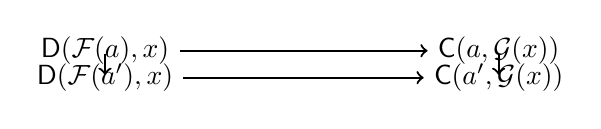
\begin{tikzpicture}[node distance={5cm}, thick, main/.style = {draw=none}]
            \node[main] (1)                 {\(\textsf{D}(\mathcal{F}(a), x)\)};
            \node[main] (2) [right of=1]    {\(\textsf{C}(a, \mathcal{G}(x))\)};
            \node[main] (3) [below=1]       {\(\textsf{D}(\mathcal{F}(a'), x)\)};        
            \node[main] (4) [right of=3]    {\(\textsf{C}(a', \mathcal{G}(x))\)};
            
            \draw[->] (1) to (2);
            \draw[->] (3) to (1);
            \draw[->] (3) to (4);
            \draw[->] (4) to (2);
        \end{tikzpicture}
    \end{center}
\end{frame}

\begin{frame}

    And, the naturality condition for \(x \to x'\) gives us the following
    commutative diagram:

    \begin{center}
        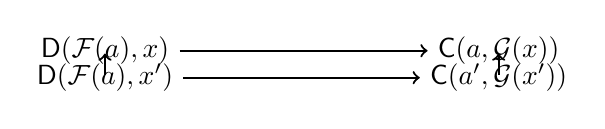
\begin{tikzpicture}[node distance={5cm}, thick, main/.style = {draw=none}]
            \node[main] (1)                 {\(\textsf{D}(\mathcal{F}(a), x)\)};
            \node[main] (2) [right of=1]    {\(\textsf{C}(a, \mathcal{G}(x))\)};
            \node[main] (3) [below=1]       {\(\textsf{D}(\mathcal{F}(a), x')\)};        
            \node[main] (4) [right of=3]    {\(\textsf{C}(a', \mathcal{G}(x'))\)};
            
            \draw[->] (1) to (2);
            \draw[->] (1) to (3);
            \draw[->] (3) to (4);
            \draw[->] (2) to (4);
        \end{tikzpicture}
    \end{center}

\end{frame}

\begin{frame}
    
We now check the adjuction between \(frg\) and \(disc\) as  defined previously.
Let \(X \) be any set and \((Y,\tau_Y)\) be any topological space. We have to
prove that 
\begin{equation}
    \cat{Top}(\textit{disc}(X) , (Y, \tau_Y)  ) \bijec \cat{Set}(X, Y)
\end{equation}
This bijection is given by  \(f \mapsto f \) in both directions. We now have to
simply check whether the two sets are the same. This is done as follows: 
\begin{equation}
    \cat{Top}(\textit{disc}(X) , (Y, \tau_Y)  ) \subseteq \cat{Set}(X, Y)
\end{equation}
is obvious since continuous functions are functions between the sets. 
\end{frame}
\begin{frame}
    
Next, note that 
\begin{equation}
    \cat{Set}(X, Y) \subseteq \cat{Top}(\textit{disc}(X) , (Y, \tau_Y)  )
\end{equation}

\begin{proof}
    Let \(f \in \cat{Set}(X,Y)\),  \(U_Y\) be any open set on \(\tau_Y\).
    \(f^{-1}(U) \subseteq X \in 2^X\) and hence \(f\) is continuous. \\
    Thus we have proved that the two sets are equal. Finally we make note of the
    naturality condition. This holds because composition of functions and
    composition of continuous function commute with the functors. 
    % explain this more clearly
\end{proof}
\end{frame}
\begin{frame}

    Given \(h \in Set(X, X')\) and \(j \in Top((Y,\tau_Y), (Y',\tau_{Y'}))\),
    
    \begin{center}
        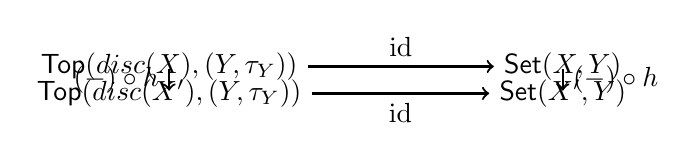
\begin{tikzpicture}[node distance={5cm}, thick, main/.style = {draw=none}]
            \node[main] (1)                 {\(\textsf{Top}(disc(X), (Y,\tau_Y))\)};
            \node[main] (2) [right of=1]    {\(\textsf{Set}(X, Y)\)};
            \node[main] (3) [below=1]       {\(\textsf{Top}(disc(X'), (Y,\tau_Y))\)};        
            \node[main] (4) [right of=3]    {\(\textsf{Set}(X', Y)\)};
            
            \draw[->] (1) to node [midway, above] {id} (2);
            \draw[->] (3) to node [midway, left] {\((-)\circ h\)} (1);
            \draw[->] (3) to node [midway, below] {id} (4);
            \draw[->] (4) to node [midway, right] {\((-)\circ h\)} (2);
        \end{tikzpicture}
        \\ \phantom{1}\\
        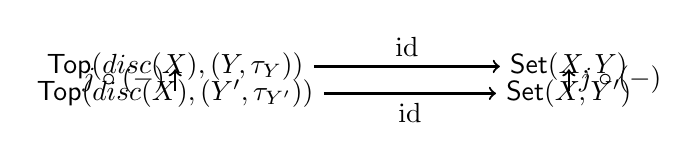
\begin{tikzpicture}[node distance={5cm}, thick, main/.style = {draw=none}]
            \node[main] (1)                 {\(\textsf{Top}(disc(X), (Y,\tau_Y))\)};
            \node[main] (2) [right of=1]    {\(\textsf{Set}(X, Y)\)};
            \node[main] (3) [below=1]       {\(\textsf{Top}(disc(X), (Y',\tau_{Y'}))\)};        
            \node[main] (4) [right of=3]    {\(\textsf{Set}(X, Y')\)};
            
            \draw[->] (1) to node [midway, above] {id} (2);
            \draw[->] (1) to node [midway, left] {\(j \circ (-)\)} (3);
            \draw[->] (3) to node [midway, below] {id} (4);
            \draw[->] (2) to node [midway, right] {\(j \circ (-)\)} (4);
        \end{tikzpicture}
    \end{center}    

\end{frame}

\begin{frame}
    
This adjunction can be restated in terms of the following universal property of
the discrete topology : The discrete topology on \(X\) is the topology such that
every function from \(X\) to any topological space \(Y, \tau_Y\) is continuous. 

\end{frame}

\begin{frame}
    Finally we take a look at the right adjoint condition for the indiscrete
    topology. The conditions states that 
    \begin{equation}
         \cat{Set}(Y,X ) \bijec \cat{Top}((Y, \tau_Y) ,\textit{indisc}(X))
    \end{equation}
    The checks are similar to the previously done checks.  We mention the only
    nontrivial check: 
    \begin{equation}
        \cat{Set}(Y,X ) \subseteq\cat{Top}((Y, \tau_Y) ,\textit{indisc}(X))
    \end{equation}
    For a given function \(f \in   \cat{Set}(Y,X )\), with the indiscrete
    topology on \(X\), \(f^{-1}(\emptyset) = \emptyset\) and \(f^{-1}(X) = Y
    \cup \emptyset\), both of which are open wrt any topology on \(Y\). Hence
    \(f\) is continuous. 

\end{frame}
